% Base TikZ Template
% Generic academic diagram starter

\documentclass[tikz,border=8pt]{standalone}
\usepackage{tikz}
\usetikzlibrary{calc,positioning,fit,backgrounds}
\usepackage{amsmath}

\begin{document}
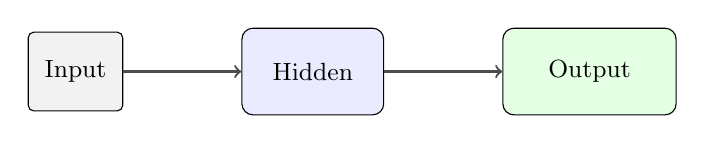
\begin{tikzpicture}[
    node distance=1.5cm,
    font=\small,
    % Node styles
    input/.style={draw, rounded corners=2pt, minimum width=1.2cm, minimum height=1cm, fill=gray!10},
    hidden/.style={draw, rounded corners=4pt, minimum width=1.8cm, minimum height=1.1cm, fill=blue!8},
    output/.style={draw, rounded corners=4pt, minimum width=2.2cm, minimum height=1.1cm, fill=green!10},
    arrow/.style={->, thick, draw=black!70},
]

    % Define nodes here
    \node[input] (in) {Input};
    \node[hidden, right=of in] (hid) {Hidden};
    \node[output, right=of hid] (out) {Output};

    % Draw connections
    \draw[arrow] (in) -- (hid);
    \draw[arrow] (hid) -- (out);

\end{tikzpicture}
\end{document}
